\chapter{Building a Linear Actuator}
\label{ch:actuator}
\paragraph{Introduction}
In order to test the glyph tracking system with repeatable motion, a linear motion system was needed. After trying a very powerful electronic linear actuator originally used for antenna movement, it was concluded to be too slow for any practical use in testing the glyph tracking system. In the matter of an evening, a simple, remotely operated and fully functional linear actuator was built, and its build procedure follows.

\paragraph{Parts required}
A handful of items are required to build the linear actuator, most of which can be found lying around a workshop or in your desk drawer.

\begin{itemize}  
        \item 1x Microcontroller (Arduino Uno)
        \item 1x H-bridge motor controller (SN754410)
        \item 1x DC motor with pulley
        \item 1x Free pulley on rod
        \item Some prototyping wires
        \item Some wood boards
        \item Some acrylic plates
        \item A piece of thread in a loop
        \item Hot glue gun
        \item Ducttape and screws
\end{itemize}

\paragraph{Build procedure}
\begin{enumerate}  
        \item The wood board is cut to wished length and a base is built using screws.
        \item Free pulley and DC motor with pulley are glued/drilled in place on the board.
        \item Electronic circuit is put together with H-bridge getting power from a stand-alone supply. We use an extra USB-port which can deliver up to 500 mA 5 volt.
        \item The Arduino Uno is programmed to trigger the H-bridge depending on input commands from the serial port.
        \item The thread is tightened until friction makes it move with load.
        \item A piece of thread is attached, that holds the payload. In our case, a laminated glyph symbol.
        \item Acrylic plates are bent to protect the pulley and thread path. Use a propane burner or other gas burner to heat up the plastic in order to bend it.
        \item Two thin pieces of wood can help in giving the glyph a smooth path to move along, and these are screwed onto the main board if needed.
        \item Ducttape and hot glue gun. The ducttape is used for construction reinforcement as well as reduction of friction so that the glyph can be pulled by the weak motor. The glue gun is used to fix some wires and further reinforce joints.
\end{enumerate}

The bottom assembly with electronics can be viewed in figure \ref{fig:bottom_asm}. This includes an acrylic bend to hold the glyph as it rests on the bottom. The electronics are rapidly put together and glued in place where applicable. The DC motor is hiding behind the duct tape. Two sets of cables are exiting the frame on the left side, one is the USB UART cable that also powers the Arduino Uno, while the other one is a pair of red-black wire that carries power from another USB port, which is used by the DC motor.

The top assembly and slider can be viewed in figure \ref{fig:top_asm}. The duct tape is used to reduce friction on the wood, so that the laminated glyph can translate without problems.

\begin{figure}[ht]
    \centering
    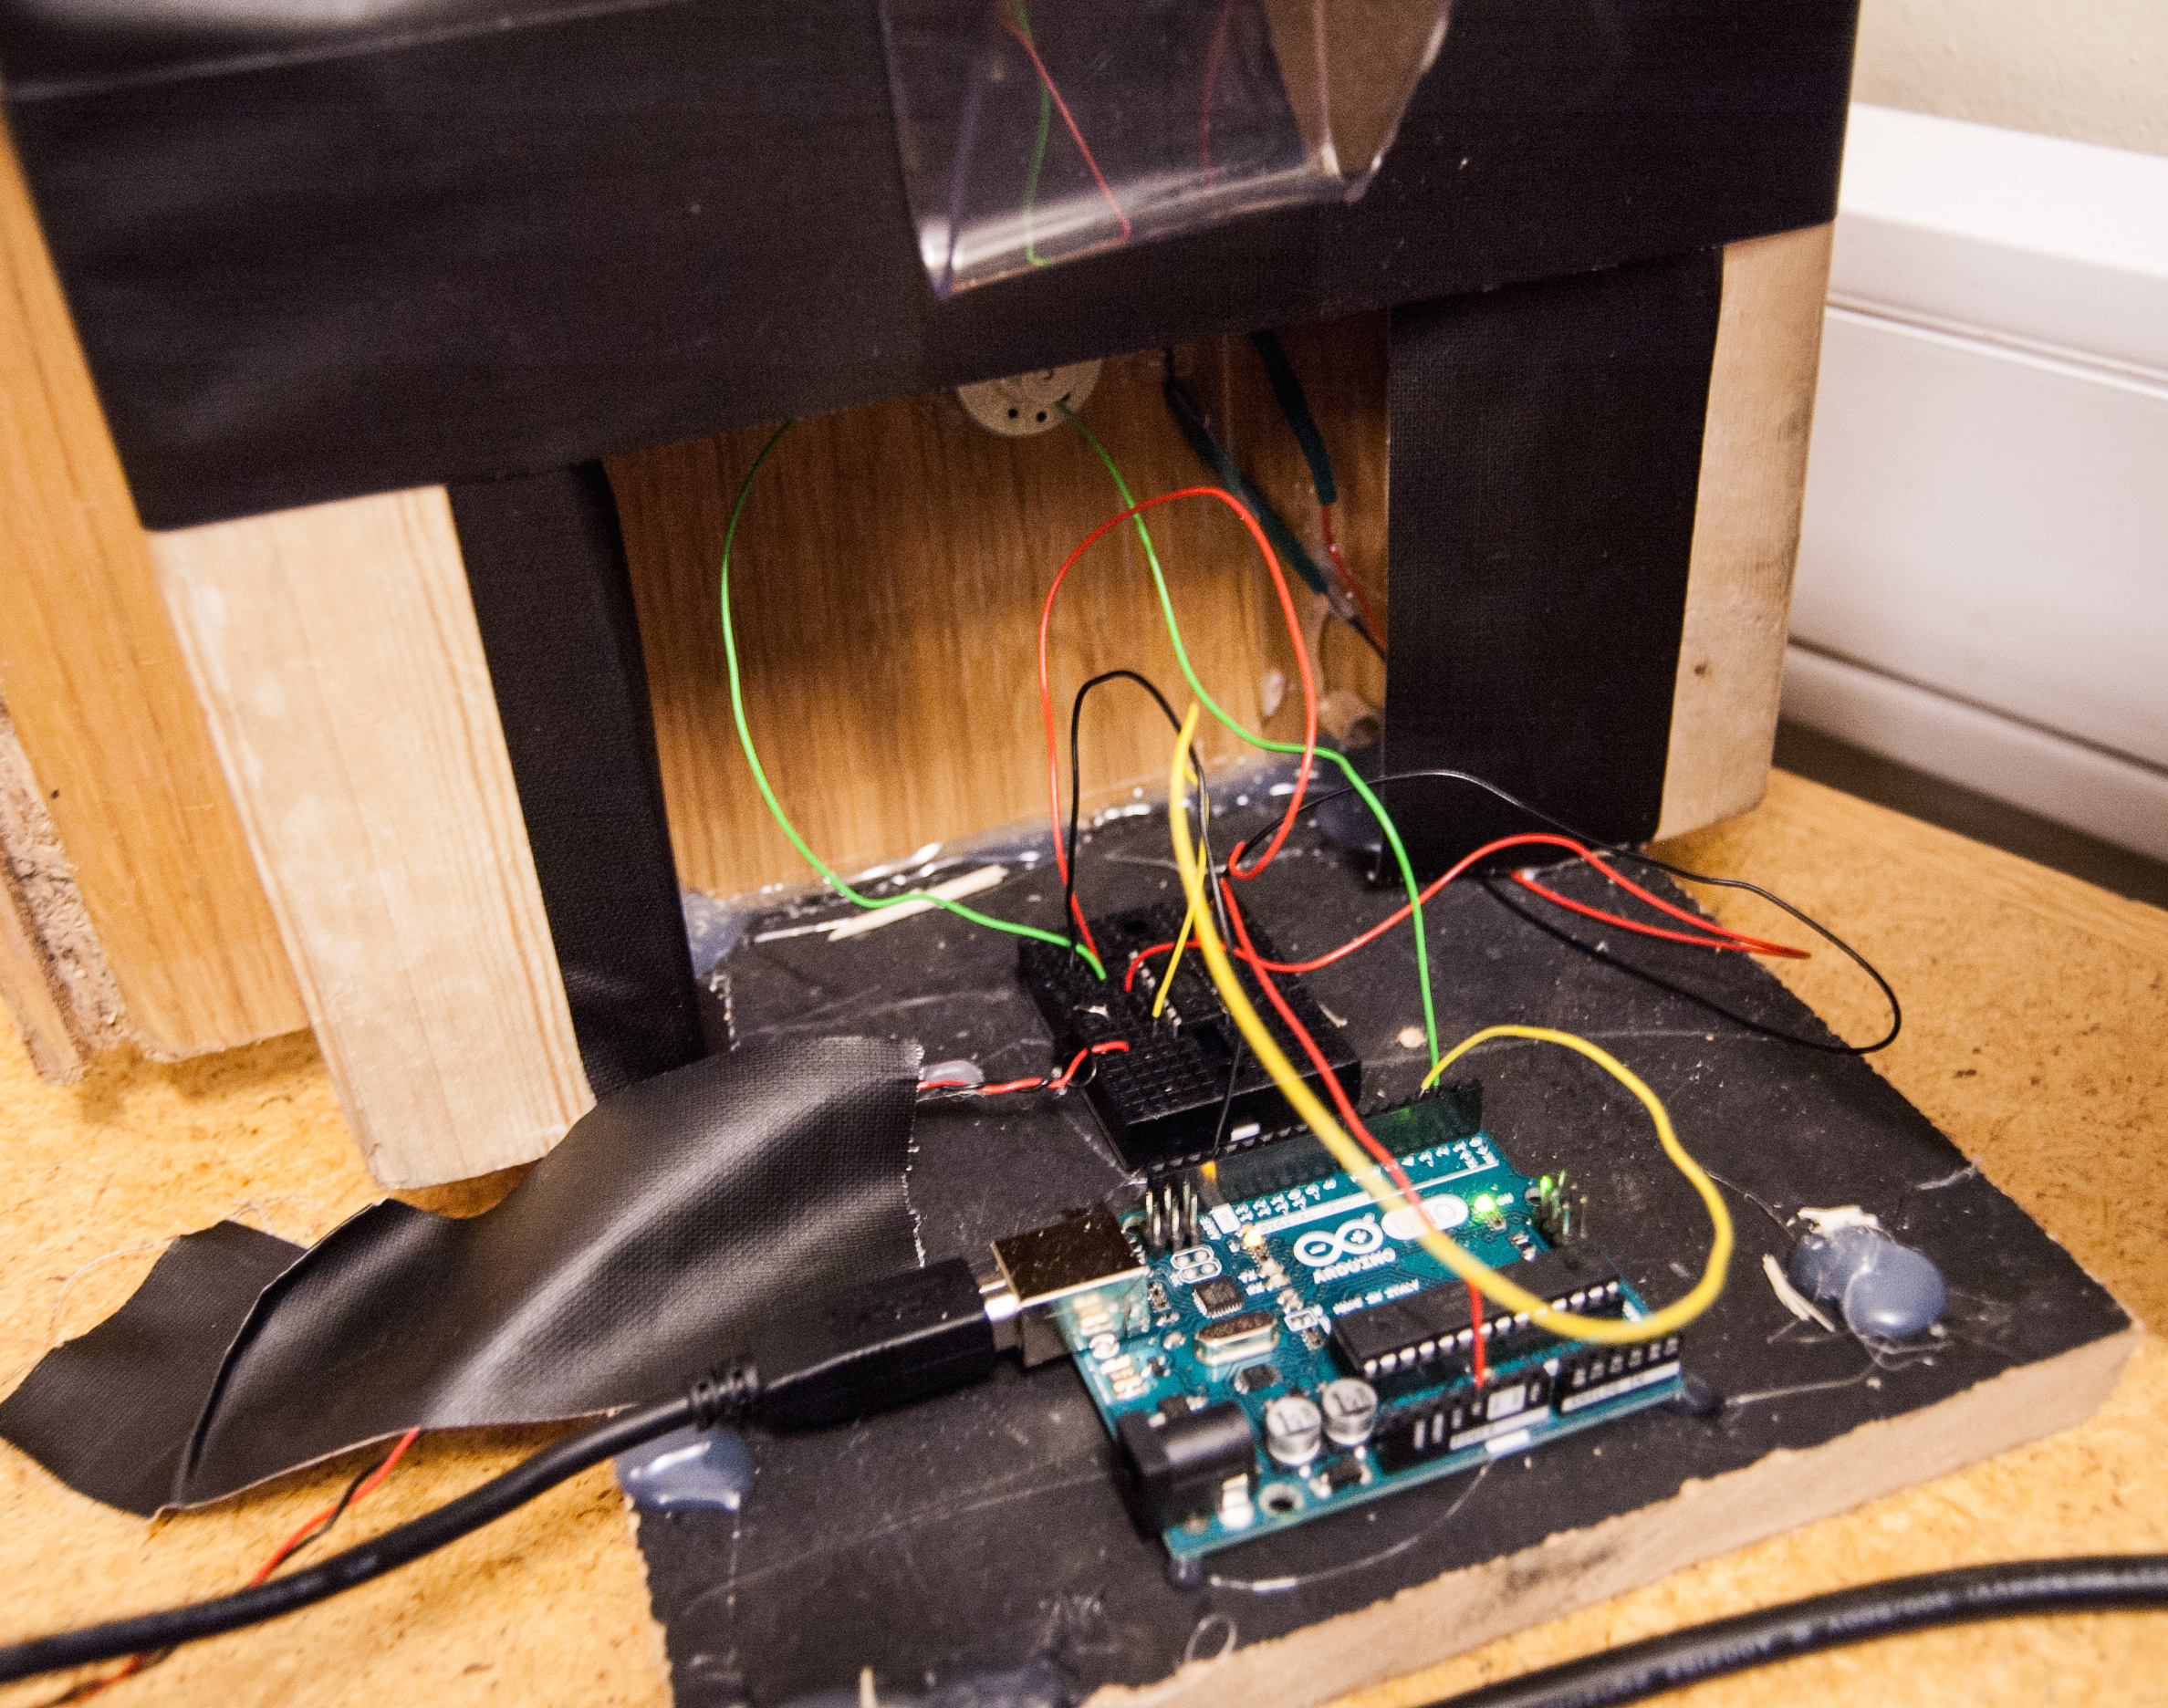
\includegraphics[width=0.8\textwidth]{bottom_asm.jpg}
    \caption{Bottom assembly. Source: Own work}
    \label{fig:bottom_asm}
\end{figure}

\begin{figure}[ht]
    \centering
    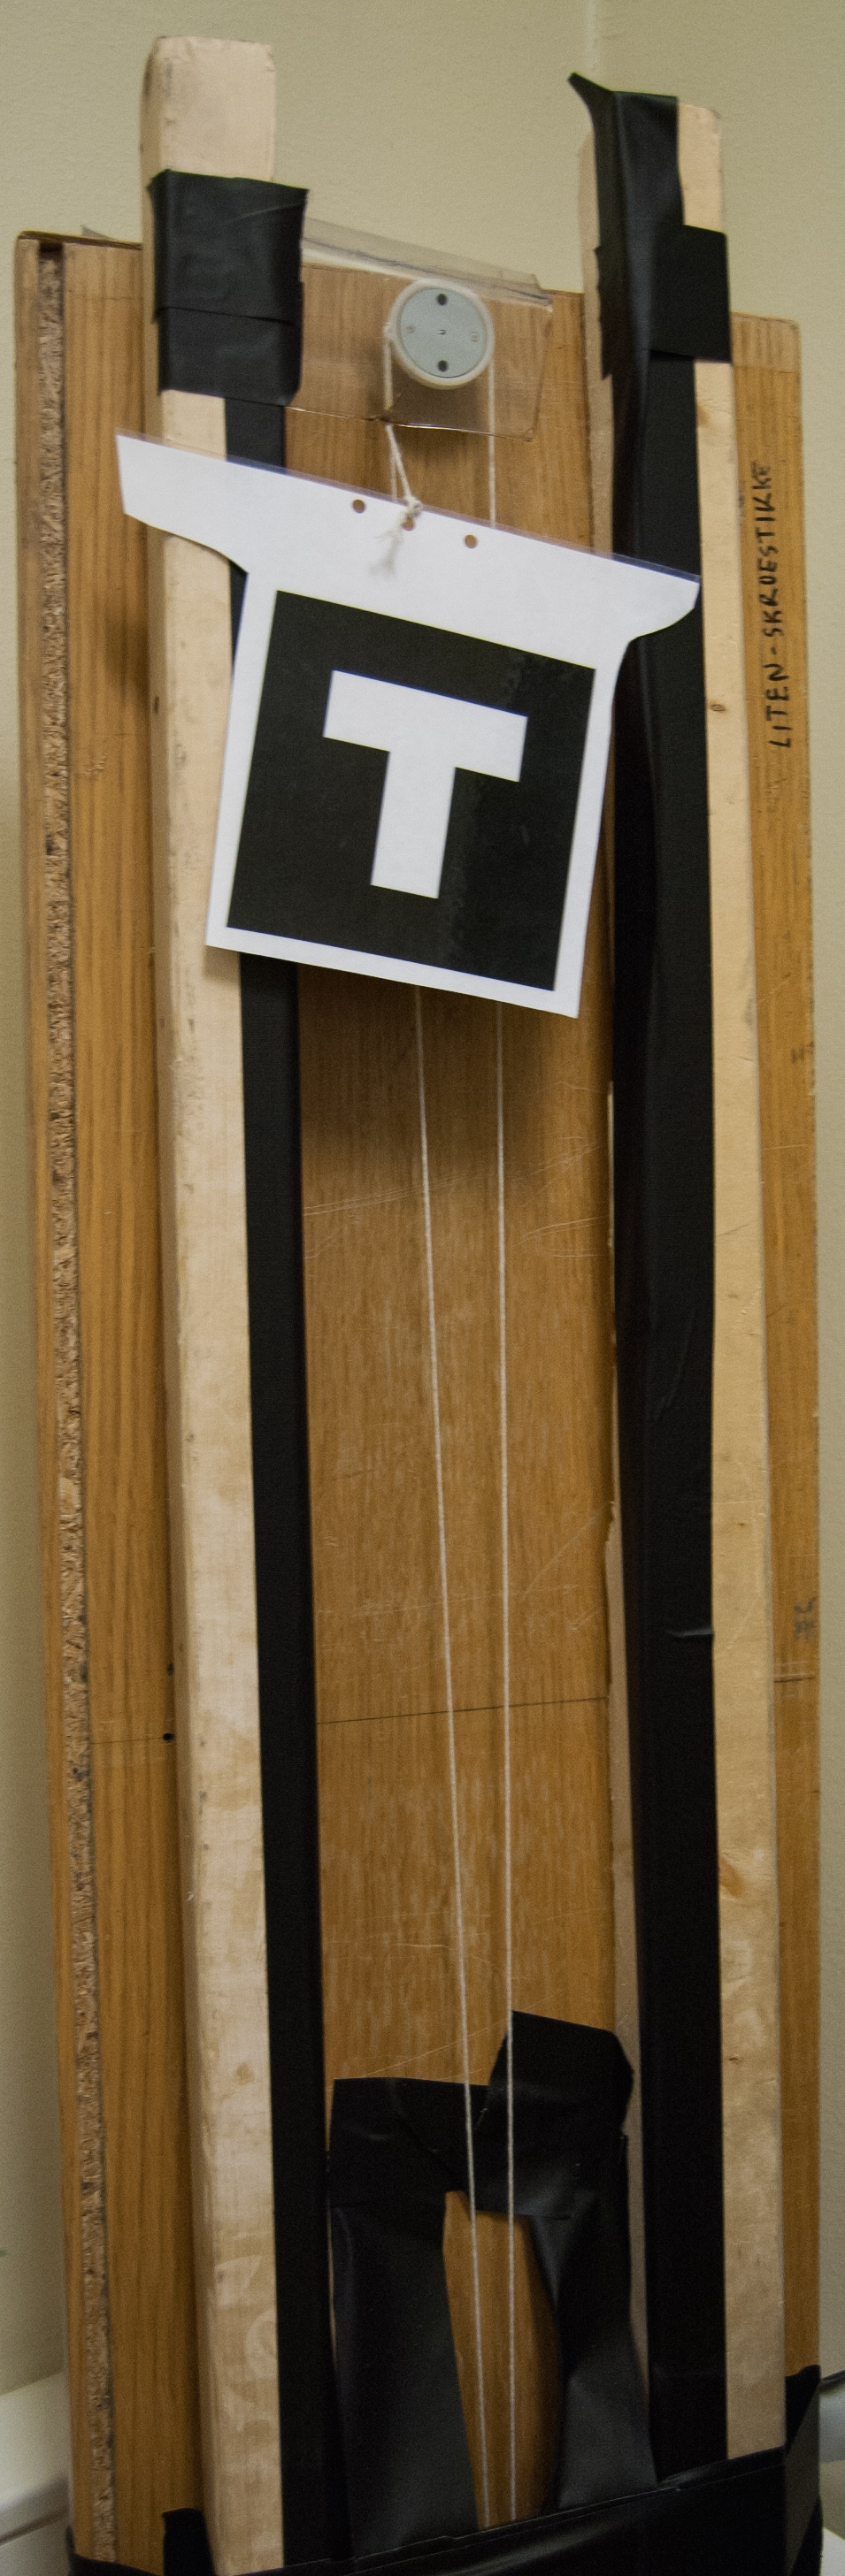
\includegraphics[width=0.4\textwidth]{top_asm.jpg}
    \caption{Top assembly and main slider. Source: Own work}
    \label{fig:top_asm}
\end{figure}
\FloatBarrier

\paragraph{Operation}
Since we are using a micro-controller board with built-in support for UART over USB, we can send commands to the linear actuator. By remotely connecting to the Linux server using SSH, we are able to test the system from anywhere in the world. See figure \ref{fig:vertical_actuator} for full communication channel.

The DC motor is too powerful to be run from the Arduino Uno 5 volt rail, it is advisable to use another power source, which feeds the H-bridge.

\begin{figure}[ht]
    \centering
    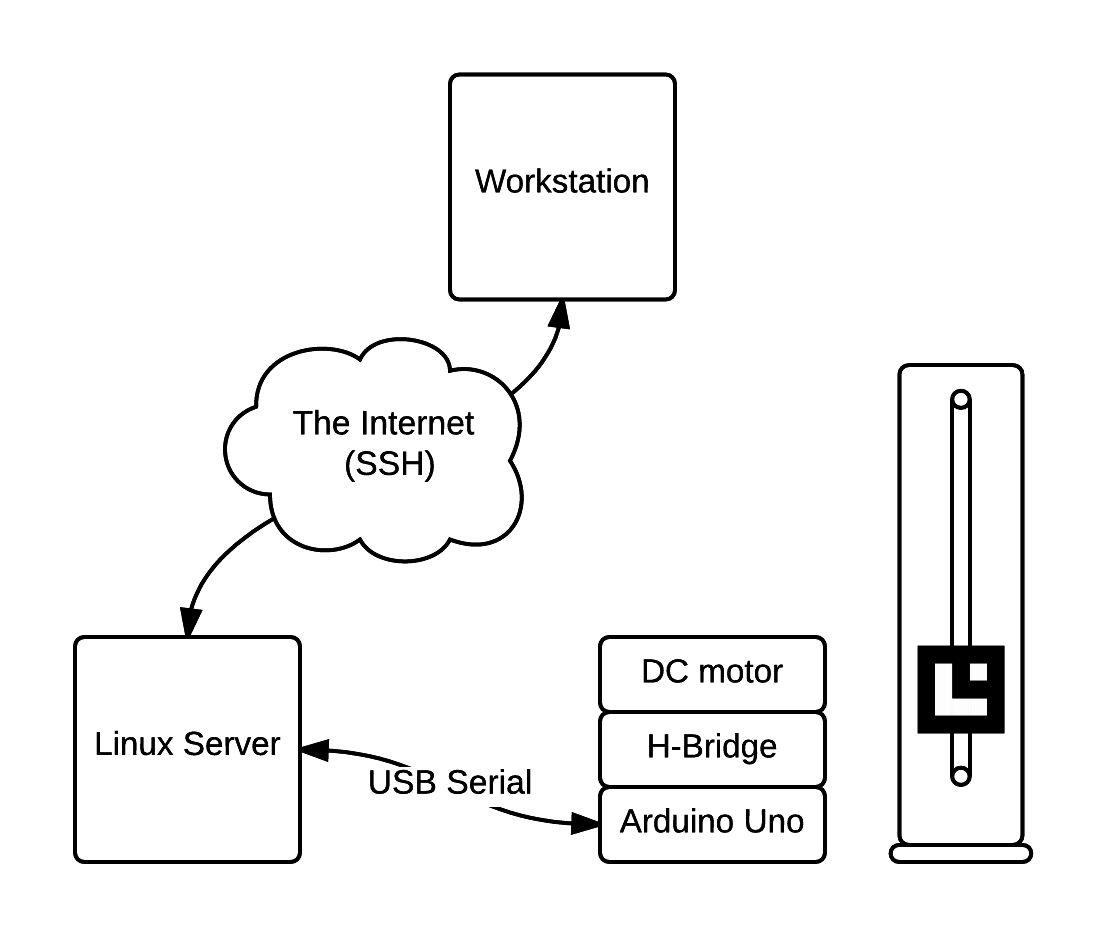
\includegraphics[width=0.8\textwidth]{vertical_actuator.png}
    \caption{Diagram over communication channel and system. Source: Own work}
    \label{fig:vertical_actuator}
\end{figure}
